\chapter{Auswertung / Experiment / Vergleich mit Property-based Testing}
\label{experimente}

\section{Vergleichmetriken}
Bevor wir einen tatsächlichen Vergleich beider Methoden durchführen werden erst einmal die Metriken eingeführt in denen
sich Verglichen wird.
Hierdurch wird einfacher verständlich welche Punkte miteinander verglichen werden.
Wir werden einige neue Metriken einführen aber auch Metriken nutzen die in \textit{Property-based Testing}\cite{property-based-testing} genutzt wurden.

\subsection{Metriken aus Property-based Testing}

In \textit{Property-based Testing} wurden zwei Metriken eingeführt, um die Methode zu evaluieren.
Hierbei wurden zwei Forschungsfragen entwickelt.

\begin{enumerate}
    \item Welche Schema Coverage kann mit der Methode erreicht werden? \cite[vgl. RQ1]{property-based-testing}
    \item Wie gut ist die Fehlerfindungskapazität der Methode? \cite[vgl. RG2]{property-based-testing}
\end{enumerate}
\caption{Forschungsfragen aus Property-based Testing}

Zur Auswertung der Methode wurden zwei Testsysteme genutzt.
Das erste Testsystem ist eine eigens entwickelte GraphQL-API die bekannte Fehler besitzt \cite[vgl. A.1]{property-based-testing}.
Testsystem 2 ist GitLab.
Ein häufig genutztes Tool für GitServer mit DevOps Kapazitäten.
Gitlab bietet seine API auch als GraphQL an und durch seine riesige Größe eignet sich GitLab als solides Testsystem. \cite[vgl. A2]{property-based-testing}
Unser entwickelter Prototyp soll in exakt dem gleichen Umfeld seine Tests generieren.
Wir erwarten, dass wir möglichst die selben Fehler finden wie die ursprüngliche Methode und positiv wäre, wenn wir mehr und neue Fehler finden würden.
Beide Forschungsfragen werden im folgenden nocheinmal näher erläutert da diese ein wenig spezialisiert sind und Wissen über Methode
ist wichtig um die Ergebnisse korrekt einordnen zu können.

\subsection{Fehlerfindungskapazitäten}

Mit Fehlerfindungskapazitäten ist gemeint wie zuverlässig die Methode tatsächliche Fehler findet.
Hierfür werden die beiden zuvor benannten APIs getestet und es wird geprüft ob die Methode die Fehler finden konnte.
Um zu verifizieren, dass die Methode möglichst viele Fehler findet gibt es eine Test API die
initial mit bekannten Fehlern versehen wird.
Die \textit{Property-based Methode} hat 11 von 15 Fehlern im speziell vorbereiteten System gefunden.
Bei GitLab wurden 15 bugs gefunden.
Unsere entwickelte Methode soll mindestens die gleichen Fehler finden und idealerweise mehr.

\subsubsection{Schema Coverage / Schema (Ab)Überdeckung}

Dadurch, dass \textit{Property-based Testing} auf zufallsbasierter Testgenerierung basiert stellt sich hier die Frage, wie gut die Methode
die API abdeckt und inwiefern die generierten Tests ausreichend sind.
Dies kommt insbesondere zu tragen, wenn die maximale Pfadlänge ausgehend vom Query Knoten größer ist als die erlaubte Rekursionstiefe des Prototypens.
In Property-based Testing wird definiert, dass die generierten Tests eine Full-Schema Coverage erreichen, wenn gilt:

\begin{definition}
    Für alle Objekte des Schemas: Bilde alle Tupel \{Object, Field \}.
    Ein Schema hat eine ideale Coverage wenn alle Tupel durch einen Test abgedeckt sind.
\end{definition}

Wie in Property-based Testing schon erwähnt: \textit{da keine Coverage Metric für GraphQL Blackbox Test Auswertung exisitiert, starten wir mit einem sehr
einfachen und intuitiven Ansatz}~\cite[vgl. B. Measuring Schema Coverage]{property-based-testing}.
In der Tat ist das vorgestellte Coveragekriterirum ein sehr einfaches Kriterium.
Es lässt zum Beispiel die Beziehungen zwischen allen Knoten aus und beachtet nur, dass alle Knoten inbegriffen sind mit allen Feldern.
Hiermit entspricht das definierte Coverage-Kriterium einer Kombination aus Edge- und Nodecoverage.
Denn alle Knoten müssen abgedeckt sein und alle Kanten ausgehend von den Knoten.
Wie zuvor gesehen ist ein solches Kriterium allerdings noch nicht ausreichend für eine ideale Testabdeckung, da
zum Beispiel die verschiedenen Kantenkombinationen außer acht gelassen werden und sich somit doch noch Fehler im Code befinden können.
Wesentlicher Unterschied beider Methoden ist insbesondere, dass \textit{Property-based Testing} überprüfen muss ob es diese Coverage erreicht.
Unsere vorgestellte Methode stellt sicher, dass diese Coverage erreicht ist bevor sie aufhört mit dem generieren.
Die Überprüfung der Schema-Coverage in Property-based Testing geschah durch ausprobieren.
Hierbei wurde ausprobiert wie viele Testgenerierungen benötigt wurden, um das definierte Kriterium zu erfüllen.
Um ein 100\% Coverage beim GitLab Schema zu erreichen waren verschiedene Anzahlen an Iterationen nötig bei verschiedenen Rekursionslimits.
Eine 100\% Coverage wurde bei GitLab nur erreicht wenn 10000 Tests mit Rekursionslimit 4 erstellt wurden.
Die Berechnungszeit war hierbei 931 Sekunden.
Dies ist zwar der schlechteste Wert in der gesamten Statistik und man könnte meinen, dass der Vergleich
nun nicht genau wäre - allerdings ist dies auch der einzige Wert der verlässlich 100\% Coverage geliefert hat.
Unser Ziel ist es also, weniger als 10.000 Tests und 930 Sekunden zu benötigen um das hier definierte CoverageKriterium zu erfüllen.

\subsection{Neue Metrik}

Näheres betrachten des Codes von \textit{Property-based Testing} offenbarte einen signifikanten Fehler in der Definition der Schema Coverage.
Hierbei ist besonders wichtig zu wissen, wie GraphQL unter der Haube funktioniert.
GraphQL verarbeitet die Schritte einer Query sequentiell.
Nutzen wir die zufällig generierte Query aus \textit{Property based Testing Fig. 9}\cite{property-based-testing}.
Die Query lautet:
\begin{lstlisting}[language=GraphQL]
    {projects(id: "7x8Z"){description members{name}}}
\end{lstlisting}

Stellen wir nun diese Anfrage an die API und es existiert kein $Project$ mit der id 7x8Z so hat die Funktion
einen return Value von $null$.
Ein Return Value von null bedeutet jedoch, dass GraphQL den Pfad nicht weiter auswerten wird und die Funktion des Resolvers hinter dem $members$ Feld nicht ausgeführt wird.
Diese Query würde jedoch die Coverage für die Tupel Project und Members erfüllen aus der vorigen Definition, ohne, dass diese wirklich getestet wurde.
Laut Property-based Testing wird hierdurch angenommen, dass die Query erfolgreich ist wenn die Query erfolgreich ist.
Allerdings haben wir nun ungetesteten Code der als getestet betrachtet wird.
Wir wollen nun eine Metrik einführen die überprüft wieviel der zufällig generierten Querys tatsächlich komplett getestet haben.
Hierfür wird folgende Metrik eingeführt:

\begin{definition}
    Für alle Querys und dazugehörigen Responses wird die Pfadlänge bestimmt.
    Eine erfolgreiche Query hat dann zwei mögliche Szenarien:
    \begin{enumerate}
        \item Pfadlänge(Query) = Pfadlänge(Response)
        \item Pfadlänge(Query) > Pfadlänge(Response)
    \end{enumerate}
\end{definition}

Tritt Fall 1 ein so hat die Query wirklich alle Funktionen getestet.
Tritt Fall 2 ein so hat die Query nicht alle Funktionen getestet.
Zählt man nun alle Querys zusammen kann man auswerten zu wieviel Prozent die gesamte erwartete Pfadlänge tatsächlich ausgeführt wurde indem die Pfadlänge(Response) hinzugezogen wird.

\section{Threats to Validity / Limitierungen}

Bevor wir mit dem eigentlichen Vergleich beginnen muss noch kurz eingeordnet werden inwiefern die Experimente zu betrachten
sind und unter welchen Vorraussetzungen der Vergleich geschieht.

\subsection{Argumentgeneratoren}

Wie in $8.1.3$ angesprochen ist es wichtig, dass GraphQL für jede Funktionen einen Wert ungleich $null$ bekommt, sodass der
Pfad weitergegangen werden kann und die Funktionen in diesem getestet werden.
Um Bedingungen zu begünstigen werden die Argumentgeneratoren für jedes Experiment angepasst, sodass es sehr viel wahrscheinlich ist, dass
die generierten Argumente auch zum SUT passen und die allgemeine Query-Qualität hierdurch besser wird.
Es hängt dann explizit davon ab wie sehr die Argumentgeneratoren angepasst werden denn ein einfaches anpassen hat sich \textit{Property-based Testing}\cite{property-based-testing}
auch erlaubt.
Hierbei sei zum Beispiel erwähnt, dass eine Type $ID$ in GraphQL als String wert definiert ist, häufig in Implementierung jedoch als Zahlenstring genutz wird.
Eine beispielhafte Anpassung wäre hier nun, dass wir den Generator für den Type $ID$ so anpassen, dass er nur Argumente für  $ID$ zurückliefert die ein Zahlenwert sind
in einem gewissen Bereich der durch das SUT abgebildet wird.


\section{Fehlerfindungskapazitäten}

Zuerst wollen wir die Fehlerfindungskapazitäten des Testtool auf die Probe stellen.
Hierfür nutzen wir die beiden, zuvor benannten, Testsyteme GraphQL-Toy (eine experimentelle GraphQL-Implementierung) und GitLab in der Version 12.6.3.
Ziel ist es mindestens die Fehler zu finden die vom \textit{Property-based Testtool}\cite{property-based-testing} gefunden wurden.
Idealerweise wollen wir jedoch sogar mehr Fehler finden.

\subsection{GraphQL-Toy}

Das Testssystem GraphQL-Toy hat ein sehr simples Schema in dem nur drei $OBJECT$ Typen exisitieren.
Diese sind $Query$, $Project$ und $User$.
Das Schema hat folgende Struktur: \\
\begin{center}
    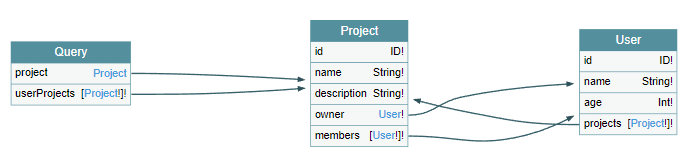
\includegraphics[width=\textwidth,height=\textheight,keepaspectratio]{img/graphqltoy}
\end{center}

Entwickelt wurde dieses System mit dem Hintergrund, dass bekannte Bugs im Code eingebracht werden und überprüft werden kann ob das Testtool diese findet.
Insgesamt wurden 15 verschiedene Buggs vorgestellt welche in verschiedene Kategorien fallen wie Syntaxfehler, falsche Rückgabedaten, falsche Datenstrukturen etc.
Einige der Bugs werden im folgenden kurz vorgestellt.
Eine Liste aller eingebauten Bugs lässt sich im Appendix unter \textit{GraphQL-Toy Implementation mit Bugs}~\ref{graphql-toy-code} finden.

\subsubsection{Bug 1 - SyntaxFehler}

Einfache Syntaxfehler wurden an verschiedenen Stellen eingebaut.
Dies bedeutet, dass jeder Funktionsaufruf dieser Funktion garantiert scheitern wird.
Somit kann jede Request diesen Fehlerfall entdecken, solange die Request auch das Feld hinter der Funktion mit dem Syntaxfehler abfragt.
Ein einfacher Syntaxfehler wäre zum Beispiel folgender Code: \\

\begin{lstlisting}[language=javascript]
    const resolvers = {
        Query: {
            project: (_, {id}, context, info) => {
                // Example bug 1 - Syntax mistake
                return db.projects.find(project => project.id ===);
            }
        }
    }
\end{lstlisting}

Hierbei fehlt der Wert mit dem die $project.id$ verglichen werden soll.
Ein jeder Aufruf dieser Funktion mit egal welcher $ID$ führt zu einem Fehler.

\subsubsection{Bug 2 - Falscher Objekttyp}

Objektfehler sind ein wenig unoffensichtlichere Fehler.
Hierbei gibt der Code ein Objekt zurück, dass nicht der definierten Struktur im Schema entspricht.
GraphQL wird hierfür dann einen Fehler erzeugen da die Daten eben nicht zum Schema passen.

\begin{lstlisting}[language=javascript]
    const resolvers = {
        Query: {
            project: (_, {id}, context, info) => {
                // Example bug 5 - wrong type "error"
                return { ...db.projects.find(project => project.id === id), name: ["a", "b"] };
            }
        }
    }
\end{lstlisting}

Um diesen Fehler ausführen zu können ist es wichtig, dass das Feld auch abgefragt wird.
Sollte das Feld ein Argument benötigen, so muss dieses passen, sodass auch wirklich ein Objekt abgefragt wird und dann der falsche Type zrückgegeben wird.

\subsubsection{Bug 3 - Typfehler in der Eingabe}

Felder wie $ID$ sind im GraphQL-Standard als einzigartige Strings definiert.
Im allgemeinen wird der $ID$ Type jedoch von diversen Entwicklern als Zahlenstring genutzt.
Eine Funktion wandelt diesen String dann in eine Zahl um die z.B. genutzt wird um einen bestimmten Eintrag eines Arrays zu bekommen.
Inputvalidierung ist also von Nöten.

\begin{lstlisting}[language=javascript]
    const resolvers = {
        Query: {
            project: (_, {id}, context, info) => {
                // Example bug 3 - Input type validation bug
                return db.projects[id];
            }
        }
    }
\end{lstlisting}

Es ist hier möglich, ohne jegliche Prüfung einen Key anzugeben.
Ist ein Resolver wie heir implementiert so ist es erlaubt in der Query jeglichen String anzugeben.
Es fällt also sehr leicht, dass z.B. ein IndexOutOfBound Fehler auftreten kann.
\\
\\
\\
\\

Mit dem Testtool nach~\cite[Property-based Testing]{property-based-testing} konnten 73\% der Fehler, also 11 der 15 Fehler gefunden  werden.
Unser entwickeltes Testtool schaffte auf der selben API auch eine Entdeckung von 11 Fehlern.
Wir konnten also dieselbe Abdeckung erreichen wie das Property-based Tool.
Bemerkenswert hierbei ist allerdings, dass das Property-based Tool hierfür wesentlich mehr Queries benötigte, um eine zufriedenstellende
Coverage zu erreichen.
Das Property-based Tool benötigte 30 Durchläufe, die jeweils bis zu 100\% Edge-Coverage liefen um alle Fehler zu finden.
Im Kontrast dazu konnte unsere hier entwickelte Methode mithilfe von nur 2 PrimePfaden eine PrimePath Coverage erreichen.
Hierzu wurden für jeden Pfad 5 Testquerys entwickelt.
Es war somit möglich, alle 11 Fehler mit nur 10 Querys zu finden. Mehr noch, im allgemeinen haben, durch die spezielle Struktur des SUT's
rein theoretisch nur 2 Querys ausgereicht, welche gut geeignet Argumente aufwiesen.
Eine Query ist gut geeignet wenn gilt, dass die erwartete Pfadlänge = wirkliche Pfadlänge.
Das Testtool fand diese beiden Querys hierfür: \\

\begin{lstlisting}[language=GraphQL]
    { project(id: "2", ) {  id  name  description   owner {  id  name  age   }  }  }
\end{lstlisting}

\begin{lstlisting}[language=GraphQL]
    { userProjects(id: "1") { name owner { id name age projects { name description id } } } }
\end{lstlisting}

Mithilfe dieser beiden Querys konnte jeder der 11 entdeckten Fehler gefunden werden.
Dies liegt auch daran, dass der Argumentgenerator entsprechend angepasst wurde und nur valide IDs produziert hat.
So war es sehr wahrscheinlich, dass eine ID die Generiert wird mindestens in einer der 5 erstellten Querys zur unterliegenden Datenstruktur gepasst hat
und wir somit die eine tatsächliche Testausführung haben und nicht nur einen initialen $null$ Wert der die Query sofort erfolgreich sein lässt.
Die 4 nicht gefundenen Fehler sind die selben Fehler wie diese, die \textit{Property-based Testing} \cite[vgl. RQ.2]{property-based-testing} nicht finden konnte.
Dies sind die Felder, in denen ein falscher Wert eines Objektes genutzt wurde um ein anderes Objekt zu erlangen.
Hierbei verhindert der Black-Box Ansatz, dass der Fehler gefunden wird.
Hierzu jedoch später mehr.

\subsection{Auswertung GraphQL-Toy}

Von den 15 injezierten Bugs wurden von beiden Tools jeweils 11 gefunden.
Die injizierten Bugs klassifizierten sich in Syntax-Bug, Validierungs-Bugs, Filtering-Bug und Wrong-Type-Bug. \cite[vgl. RQ 2 Type Errors]{property-based-testing}.
In \textit{Property-based Testing} fand der entwickelte Prototyp 11 Bugs.
Es wurden alle Bugs gefunden die nicht in der Kategorie Filtering-Bug waren.
Bugs der Kategorie Filtering-Bug wurden nicht gefunden da diese Bugs valide 200er Statuscodes zurückgeben aber oft
leere Felder.
Da durch den BlackBox Ansatz jedoch keine Information existiert, die uns verlässlich sagen kann, dass Daten falsch sind,
werden diese Fehler akzeptiert und es wird kein Fehler erkannt.
Diese Limitierung existiert in unserem hier entwickelten Prototyp auch.
Wir haben exakt die selben Fehler finden können wie das Property-based Tool.
Da wir in unserem Prototypen auch den Ansatz BlackBox-Testing gewählt haben, haben wir mit diesem Problem auch zu kämpfen.
\\
Unser hier entwickelter Prototyp hat jedoch für die allgemeine Fehlerfindung wesentlich weniger Tests benötigt.
Das Schema des GraphQL-Toy umfasste einen sehr simplen Graphen.

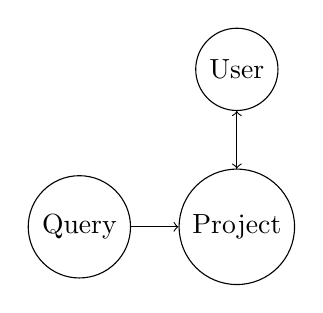
\begin{tikzpicture}
    \node[circle, draw] (n1) at (0,0) {Query};
    \node[circle, draw] (n2) at (2,0) {Project};
    \node[circle, draw] (n3) at (2,2) {User};

    \draw[->] (n1) -- (n2);
    \draw[->] (n2) -- (n3);
    \draw[->] (n3) -- (n2);
\end{tikzpicture}

Unsere Methode ermittelte zwei Pfade als ausreichend für die Testgenerierung.
Pro Pfad wurden dann 5 Tests erstellt.
Aus diesen insgesamt 10 ermittelten Tests ergaben sich dann Tests die ausreichend waren ebenso alle Fehler zu finden.
Bemerkenswert ist hier, dass das Tool nur ein einziges Mal seine Tests generieren musste.
Es wurden somit 10 Tests generiert, die fähig waren, alle Fehler zu finden.
In diesem kleinen Beispiel hat unser hier entwickelter Prototyp die selben Fähigkeiten wie der \textit{Property-based Prototyp}.
Die ausgeführten Experimente befinden sich im GitHub \cite{github-toy-experimente}.

\subsection{GitLab}

Das Testsystem GitLab wurde schon in Property-based  Testing verwandt um an einem Industry-ready Projekt die Methode zu evaluieren.
Wir wollen dies mit unserem Test-system auch durchführen.
GitLab stellt sowohl eine REST als auch GraphQL-API zur Kommunikation  zur  Verfügung.
Mit GitLab wird ein komplexes Softwareprodukt zur Versionsverwaltung und DevOps-Anwendung getestet.
Die Komplexität dieser Softwarewird deutlich, wenn wir uns das GraphQL-Schema von GitLab ansehen.
Dieses ist sehr komplex und stark zyklisch.

\begin{center}
    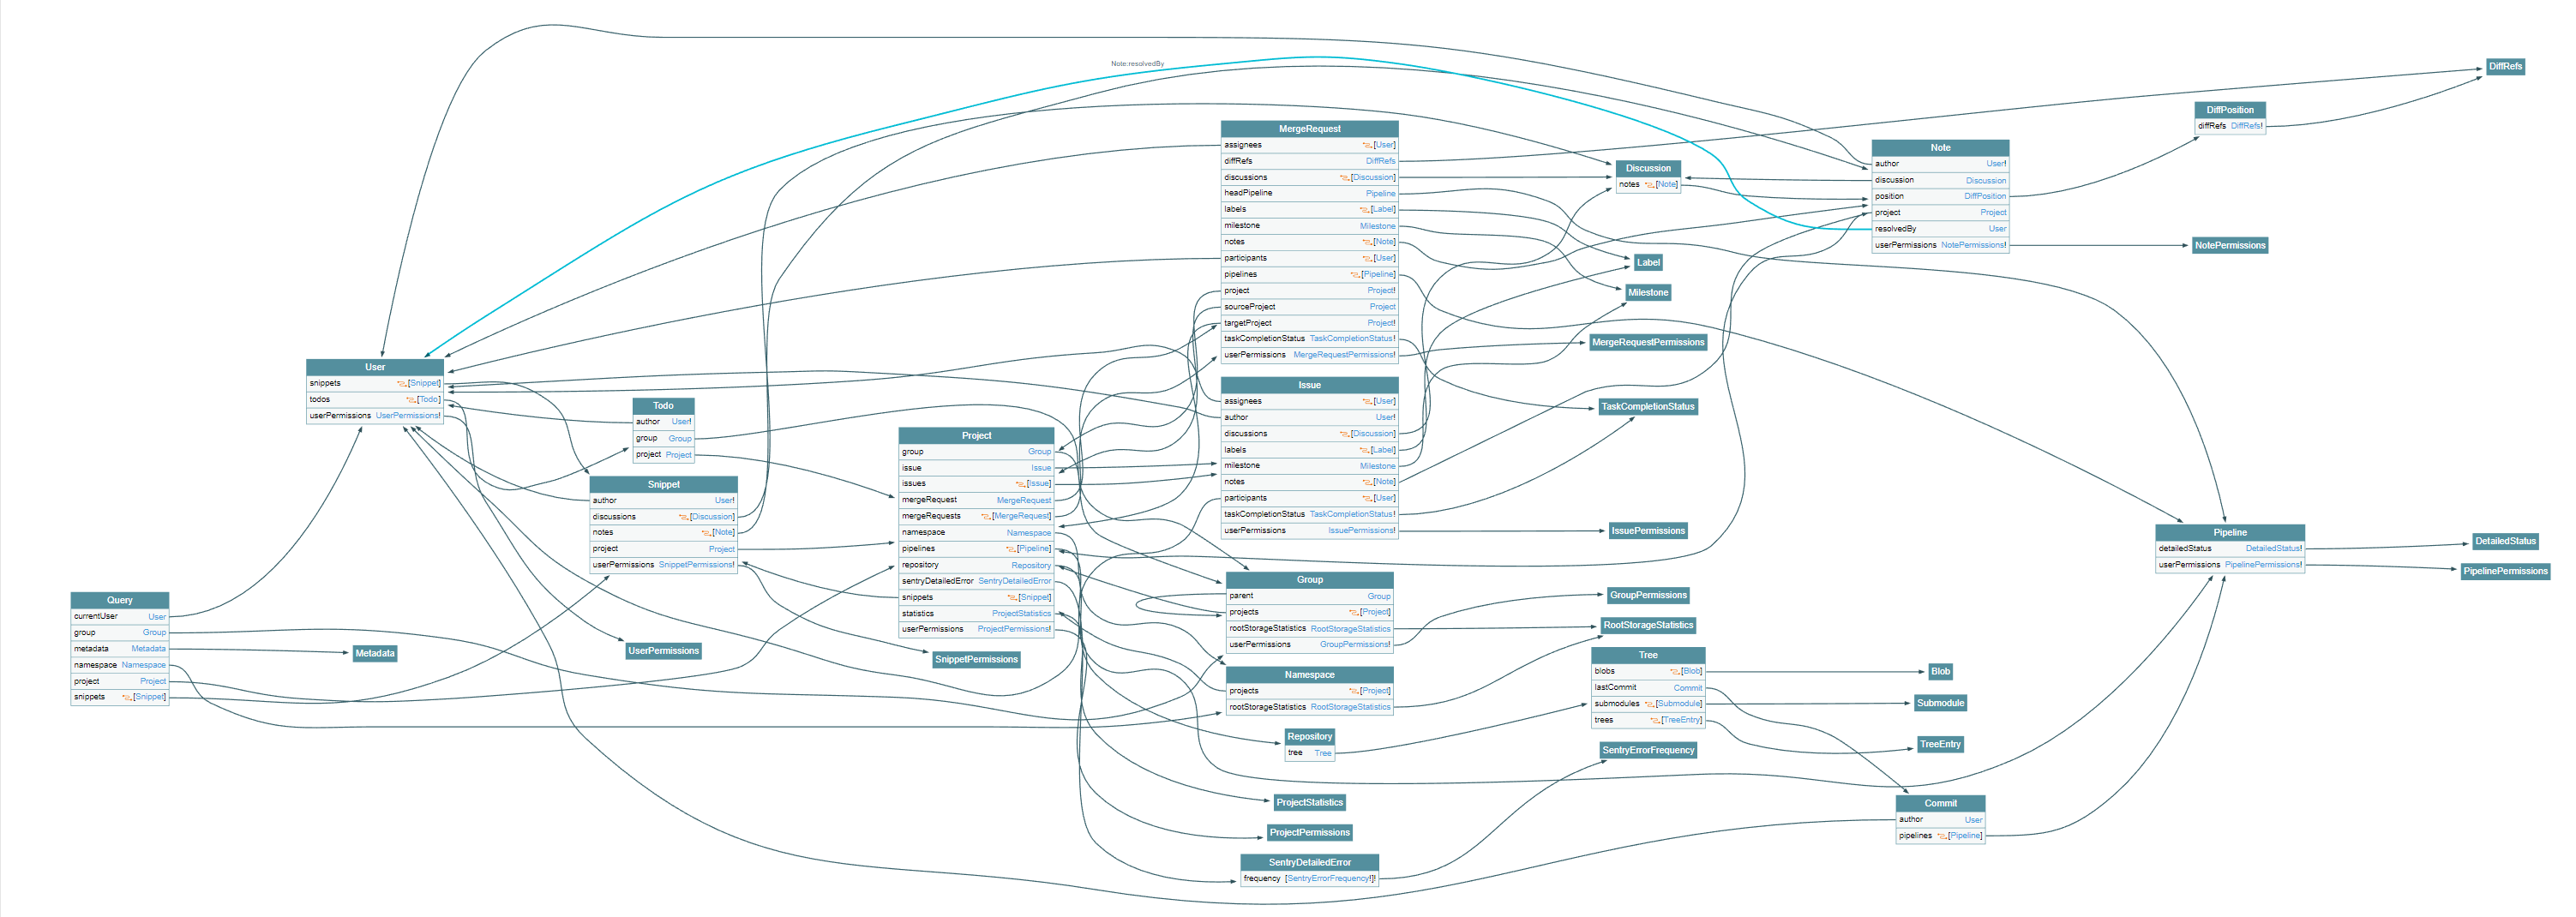
\includegraphics[width=\textwidth,height=\textheight,keepaspectratio]{img/gitlabgraph}
\end{center}

\subsection{Auswertung GitLab}

Das \textit{Property-based Testtool} fand insgesamt 4 Fehler die im Query-Bereich von GraphQL waren.
Alle Fehler waren Fehler in der Validierung von Eingabevariablen.
Hierbei lag der Fehler darin, dass die Resolver einen fehler verursachten wenn als Eingabe ein String mit leerem Zeichen kam.
Dies bedeutet, ein leerer String \verb+""+ wird richtig behandelt aber ein String mit leerem Zeichen führt zum Fehler: \verb+e\u0000\+
Die Fehler wurden gefunden durch folgende Querys:

\begin{lstlisting}[language=GraphQL, caption=Fehler 1\cite{issue1}]
{project(fullPath: "root/test-project") {sentryDetailedError(id: "") {count}}}
\end{lstlisting}

\begin{lstlisting}[language=GraphQL, caption=Fehler 2\cite{issue2}]
{project(fullPath: "e\u0000") {name fullPath}}
\end{lstlisting}

\begin{lstlisting}[language=GraphQL, caption=Fehler 3\cite{issue3}]
{namespace(fullPath: "e\u0000") {fullName name fullPath}}
\end{lstlisting}

\begin{lstlisting}[language=GraphQL, caption=Fehler 4\cite{issue4}]
{group(fullPath: "e\u0000"){fullName name fullPath }}
\end{lstlisting}

Alle vom Property-based Tool gefunden Fehler wurden durch unseren Prototypen gefunden mit den Querys

\hyperref[query1]{Query 1},
\hyperref[query2]{Query 2},
\hyperref[query3]{Query 3} und
\hyperref[query4]{Query 4}.

Getestet wurde auf dem offiziellen GitLab-Docker Image in der Version 12.6.3
Damit im GitLab auch Daten verfügbar sind wurde ein Population-Skript geschrieben, dass im GitLab
50 User anlegt und jedem User einige Projekte, Commit, MergeRequests etc. zuordnet.
Das Population-Skript kann im~\cite[Github]{populationscript} gefunden werden.
Da die Querygenerierung stets im Query-Knoten beginnt und die PrimePaths gefunden werden sollen, ergeben sich in diesem
Schema sehr viele ähnliche Querys.
Diese unterscheiden sich insbesondere am Ende der jeweiligen Query.
Der zuvor vorgestellte Algorithmus errechnet für das Schema von GitLab eine Pfadanzahl von 41744 für eine
PrimePath-Coverage des Schemas.
Eine genaue Auflistung aller Pfade findet sich im~\cite[GitHub]{gitlabpaths}.
Mit der Maßgabe, dass wir pro Pfad 5 Tests erzeugen wollen wurden dann 208.720 Tests erzeugt.
Diese Große Anzahl an Tests ergibt sich allerdings auch daraus, dass der Graph der von
GraphQL erzeugt wird, einerseits wenige Einstiegspunkte hat.
So hat der Query-Type nur 5 ausgehende Felder die für tiefere Pfadbildung relevant sind, 1 Feld hat nur MetaInformationen über
die GitLab Software und erzeugt kein weiteren Pfade.
Dies bedeutet, dass jeder Pfad auch mit einem dieser Felder beginnt da wir stets
unsere Pfade aus dem Query-Type starten lassen müssen.
Die zufällige Generierung von Argumenten limitiert hier dann dementsprechend, dass Tests sehr selten unser
eingeführtes Measurement erfüllen.
In nahezu allen Fällen haben die generierten Tests eine tatsächliche Pfadlänge die kleiner ist als die erwartete.
In mehreren Durchläufen zeigte sich, dass im Schnitt nur ca. 20 Tests eine ideale Pfadlänge erreichen.
Die Tests, die das erreichen sind im allgemeinen auch Tests, die einen sehr kurzen Pfad abbilden.
Hier verringert sich einfach das Risiko, dass Eingabeargumente generiert werden, die keine zugrundeliegenden Daten haben und somit die
Pfadausführung verhindern.
Ein Beispiel hierfür ist der Pfad $Query -> Project -> MergeRequest -> Time$

\begin{lstlisting}[language=GraphQL]
{ project(fullPath: "groupx_3/projectx_2_1") {
    archived
    avatarUrl
    containerRegistryEnabled
    ...
    mergeRequest(iid: "1") {
        allowCollaboration
        createdAt
        mergeStatus
        ...
        }
    }
}
\end{lstlisting}

durch gutes Mocken des FullPath Argumentgenerators war es möglich, eine Query zu generieren, die somit passende Argumente generiert hat
um für eine ideale Testausführung (d.h. Länge Ergebniss = Länge Testpfad) zu sorgen.
Generell zeigt sich sehr schnell, dass bei unserer Methode ähnliche Limitierungen wie im Property-based Testing auftreten.
So ist eine Anpassung an das Domänenwissen nötig.
Für GitLab bedeutet dies unter anderem, dass die ID-Struktur um z.B. Projekte abzufragen in der Form \verb+<user>/<project>+ sein muss. \cite[vgl. S.8]{property-based-testing}
Da wir vom Prinzip her ähnliche Argumentgeneratoren verwendet haben wie in Property-based Testing, haben wir auch diese Limitierungen.
Wir generieren zwar sehr viele Tests die auch PrimePath Coverage ideal erreichen würden.
Wenn jedoch die Generierung der Tests auf Zufall basiert, so können wir auch nicht garantieren, dass unsere Eingabeargumente passend sind und ein valides Ergebniss zurückgeben.
Wird kein Ergebniss zurückgegeben, so folgert GraphQL, dass spätere Funktionen nicht ausgeführt werden müssen und somit werden diese auch nicht getestet.
Es ist möglich, dieses Problem zu beheben, hierzu jedoch in FutureWork mehr.

\section{Schema-Abdeckung}

Für die Schemaabdeckung wurde im Property-based Testing die Edge-Coverage als zufriedenstellendes Coveragekriterium gewählt.
Dieses Coveragekriterium findet allerdings keine Berücksichtigung in der Testgenerierung und ist in der Arbeit lediglich ein Measurement.
Mit diesem soll gezeigt werden, wie viele Tests zufällig generiert werden müssen, damit im Durchschnitt eine zufriedenstellende Abdeckung erzielt wird.
Dadurch wird die Überlegenheit bereits aus struktureller Sicht deutlich.
Während im Property-based Testing nicht garantiert wird, dass eine zufriedenstellende Coverage erreicht wird,
sichern wir durch unseren Generierungsalgorithmus zu, dass die generierten Tests der PrimePath-Coverage entsprechen.
Dies stellt ein stärkeres Coveragekriterium dar als die Nodecoverage.
Dennoch möchten wir untersuchen, wie gut die Coverage in der Praxis funktioniert.
Dafür betrachten wir erneut die beiden zuvor benutzten Beispiele: einerseits das GraphQL-Toy als minimales Beispiel und andererseits GitLab als komplexes Beispiel.
Wir betrachten die Abdeckung des Schemas eher auf theoretischer Seite.
Die Limitierung der zufälligen Argumentgeneratoren behindern eine tatsächliche Umsetzung der hier vorgestellten Methode.
Allerdings lösen sich diese auf, sobald das Problem der Argumentgeneratoren gelöst ist.

\subsection{GraphQL-Toy Schema Coverage}

Wie zuvor gesehen in $8.3.1$, ist das Schema des GraphQL-Toys ein sehr simples.
3 Knoten, 5 Kanten bilden den ganzen Graphen.
Das Property-based Tool nutzt zur Überdeckung des Graphens die Edge-Coverage. \cite[vgl. Measuring Schema Coverage]{property-based-testing}
Wie eingeführt in \textit{Property-based Testing}\cite{property-based-testing} muss für eine zufriedenstellende Coverage
die Tatsache erfüllt sein, dass jedes paar von \verb+(Type, objectField)+ abgedeckt sein.
Dies bedeutet für das Schema, dass die Felder

\begin{itemize}
    \item \verb+(Query, project)+
    \item \verb+(Query, userProject)+
    \item \verb+(Project, owner)+
    \item \verb+(Project, members)+
    \item \verb+(User, projects)+
\end{itemize}

abgedeckt sein müssen um Edge-Coverage zu erfüllen.
Da nur die beiden initialen Felder aus dem Query-Type Eingabeargumente benötigen ist die Querygenerierung relativ simpel.
Wir können keine Aussage darüber machen ob die generierten Querys von \textit{Property-based Testing}\cite{property-based-testing} diese Coverage erfüllen
denn bei der Querygenerierung spielt es keine Rolle ob dieses Measurement erreicht wird.
Es gibt lediglich eine Messung die zeigt, dass der Prototyp mit hinreichender Wahrscheinlichkeit in der Lage ist, durch zufällige Querygenerierung
Tests zu generieren, die Edge-Coverage erfüllen. \cite[vgl. D.Results RQ1 ]{property-based-testing}.
Im Gegensatz zum Property-based Testing hat der heir entwickelte Prototyp den Vorteil, dass die Pfadgenerierung nicht zufällig ist.
Wir berechnen PrimePaths, diese sind ein stärkeres Coveragekriterium als die Edge-Coverage.
Dadurch ergibt sich, dass die Tests die vom hier entwickelten Prototyp erstellt werden, stets diese Coverage erfüllen.
Die Coverage muss nun also nicht mehr durch hinreichend viele Tests sichergestellt werden.
Ein einziger Durchlauf reicht aus um sicherzustellen, dass die gewünschte Coverage erreicht ist.
Natürlich bleibt offen ob die generierten Tests diese Coverage tatsächlich erreichen jedoch ist auch ein Problem im Property-based Testing.
Dort wird auch nur geprüft, ob die Felder in der Anfrage existieren.
Um dies eben messbar zu machen haben wir in $8.1.3$ eine neue Metrik eingeführt die überprüfen soll ob die erwartete Coverage der Query mit der
tatsächlichen Übereinstimmt.

\subsection{GitLab Schema Coverage}

Das GitLab Schema ist wesentlich komplexer.
Im Gegensatz zum GraphQL Toy besteht das GitLab Schema aus 37 Knoten welche jeweils zahlreiche Kanten hinzufügen.
Generell lässt sich sagen, dass das Schema sehr komplex und stark rekursiv ist. \cite[vgl. Studied Cases 2]{property-based-testing}
Da der Property-based Testing Ansatz ein Rekursionslimit benötigt stellt sich hier die Frage inwiefern überhaupt das Schema überdeckt werden kann.
Laut Paper hat sich ein Rekursionslimit von 4 als hinreichend ausgezeichnet \cite[vgl. Table 1 ]{property-based-testing} und wurde auch so
im Code übernommen.
Ein Rekusionslimit von 4 bedeutet, dass die maximale zu erreichende Pfadlänge des Testpfades 4 ist.
Da das GitLab-Schema aber nun einen Graphen aufspannt, der durchaus wesentlich längere Pfade als 4 hat, ist es fragwürdig wie die 100\% Schema-Coverage
in \cite[Table 1]{property-based-testing} berechnet wurden.
Es seien hier einige Pfade beispielhaft genannt, die einzigartig sind, bei denen sich keine Kante doppelt und deren Länge 4 stark überschreitet: \\

\verb+Query -> User -> SnippetConnection -> SnippetEdge -> Snippet -> DiscussionConnection -> DiscussionEdge -> Discussion -> NoteConnection -> NoteEdge -> Note -> Project -> IssueConnection -> Issue -> Milestone -> Time+ \\
\verb+Query -> Project -> Issue -> DiscussionConnection -> DiscussionEdge -> Discussion -> NoteConnection -> NoteEdge -> Note -> User -> SnippetConnection -> SnippetEdge -> Snippet -> Time+ \\
\verb+Query -> Namespace -> ProjectConnection -> Project -> MergeRequestConnection -> MergeRequestEdge -> MergeRequest -> UserConnection -> User -> SnippetConnection -> Snippet -> DiscussionConnection -> PageInfo+ \\

Somit gilt, dass in Property-based Testing der Graph des GraphQL-Schemas zum Coverage-Measurement beschnitten wurde, dass nur noch zum jeweils passenden
Rekursionslimit die Pfadlänge berücksichtigt wird.
Im Grunde lässt sich sagen, dass die genannten 100\% Schema Coverage bedeuten, dass alle erreichbaren Felder mit Pfadlänge = Rekursionslimit
in den Tests berücksichtigt sind.
Dies ist ein sehr großer, struktureller Einschnitt und die in Property-based Testing genannten 100\% Edge-Coverage sind keine
100\% Edge-Coverage auf dem Scchema im eigentlichen Sinne so wie es hier erarbeitet wurde.
Die genannten 100\% Coverage sind eine Edge-Coverage für einen reduzierten Graphen der aufgrundlage der
Rekursionstiefe reduziert wird.
Wie auch zuvor erwähnt, erzeugt unser hier entwickelter Prototyp Tests die in unserem Fall die PrimePath-Coverage umsetzen.
Da PrimePath-Coverage ein stärkeres Coverage-Kriterium als Edge-Coverage darstellt, haben wir hier einen strukturellen Vorteil
der uns garantiert, dass die Coverage besser ist.
Außerdem reduzieren wir unseren Graphen nicht.
Wir führen die Pfadgenerierung auf dem gesamten Graphen aus und erhalten, wie zuvor erwähnt, über 40.000 Pfade zurück die nötig sind
um eine PrimePath-Coverage für das GitLab Schema zu erreichen.
Hier zeigt sich auch ein direkter Unterschied.
Während in Property-based Testing gesagt wird, dass 10.000 Tests mit einem Rekursionslimit von 4 ausreichen um ein 100\% Edge-Coverage zu erreichen \cite[vgl. Table 1]{property-based-testing}
so sehen wir, dass 10.000 Tests nicht reichen können wenn allein schon über 40.000 PrimePaths existieren.
Insbesondere sei hierbei angemerkt, dass die Pfad- \& Testgenerierung auf dem GitLab-Schema keine alzu komplexe Aufgabe war.
Die Berechnung der Querys geschah auf einem hardwaretechnischen ähnlichem Level wie in Property-based Testing verwandt. \cite[vgl. Experimental Setup]{property-based-testing}.
Hier wurde die Aussage getroffen, dass ein \cite[Tiefensuchen Ansatz nicht skaliert und deswegen ein iterativer Ansatz zu präferieren ist]{property-based-testing}.
Der hier entwickelte Prototyp zeigt das Gegenteil.

\section{Zusammenfassung der Experimente}

Wir konnten in beiden Experimenten zeigen, dass unser Prototyp die selben Fehler findet wie der Prototyp aus Property-based Testing.
Einige Verbesserungen konnten wir eingehen aber wir leiden auch unter ähnlichen Problem wie Property-based Testing.
Durch unseren Ansatz ist es möglich geworden, die Schema-Coverage der Tests nachweisbar zu erhöhen und wesentlich verlässlicher zu machen.
So ist im Property-based Ansatz immer ein gewisser Zufall entscheidend wie gut die Tests sind.
Die Verlässlichkeit der Abdeckung mit Tests ist hier nicht gegeben.
Hier konnten wir mit unserer neu entwickelten Methode Fortschritte erzielen indem wir zeigten, dass es möglich ist aus einem GraphQL Schema
einen Graphen zu bilden, auf diesem Coverage Algorithmen laufen zu lassen und aus den gewonnen Tests-Pfade zu ermitteln.
Somit kann der Ansatz des Property-based Testings mit unserer Methode erweitert werden und die Testcoverage verlässlich und nachweisbar erhöhen.
Limitierungen unseres Prototypen bestehen genau wie im Property-based Testing noch.
Hierbei generiert unser Tool sehr komplexe und präzise Querys die das System gut testen würden.
Allerdings werden Argumente nur zufällig generiert und verhindern somit oft, dass diese komplexen Querys vollständig ausgeführt werden.
Einerseits kann dieses Problem auf manuelle Art und Weise verbessert werden indem man die Argumentgeneratoren anpasst und diesen hilft indem
man z.B. ID-Generierungen anpasst.
Andererseits lässt sich dieses Problem wahrscheinlich auch lösen wenn man sich vom BlackBox-Testing lösen kann und die Methode weiterentwickelt, sodass
aus dieser ein Grey oder WhiteBox Testing wird.
Hierzu jedoch in futureWork mehr.











